\documentclass{article}

\pagestyle{empty}

\usepackage[margin=1in]{geometry} % Fix margins 

\usepackage{wheelchart} % Need for pie graphs

\begin{document}

\begin{center}
\LARGE{\textbf{Demographic Profile: Fulton County}}\\
\end{center}

\section*{Race and Ethnicity}

\begin{tabular}{| p{4in} || r | r | }

\hline
& \textbf{Count} & \textbf{Percent} \\
\hline
Total Population & 1,076,561 & 100\% \\ 
\hline
Non-Hispanic White & 396,329 & 37\% \\
\hline
Non-Hispanic Black or African American & 453,703 & 42\% \\
\hline
Non-Hispanic Asian & 83,505 & 8\% \\
\hline
Non-Hispanic Other & 55,057 & 5\% \\
\hline
Hispanic or Latino, All Races & 87,967 & 8\%\\
\hline


\end{tabular}

\section*{Educational Attainment}

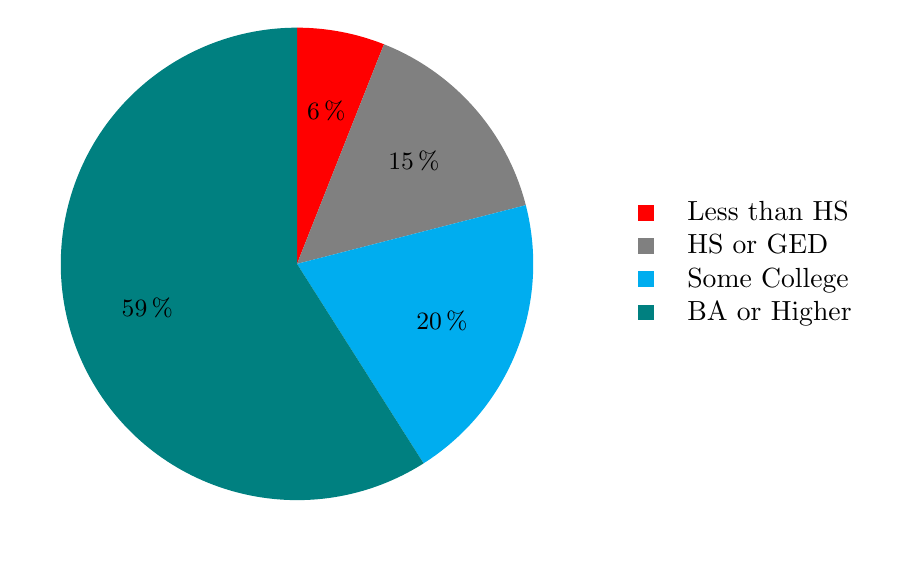
\begin{tikzpicture}
    \wheelchart[
        pie,
        radius={0}{3},
        slices style={fill=\WClistcolors, draw=none},
        WClistcolors={red, gray, cyan, teal},
        value=\WCvarA,
        % Inside Slices: Show Percentages
        wheel data=\WCperc,
        wheel data style={black, font=\small},
        % Legend: Show Labels (e.g., Less than HS)
        legend row={\tikz\fill[\WClistcolors] (0,0) rectangle (0.2,0.2); & \WCvarB},
        legend={
            \node[right] at (4,0) {
                \begin{tabular}{ll}
                    \WClegend
                \end{tabular}
            };
        },
        % Disable the default label search
        data={} 
    ]{
        6/Less than HS,
        15/HS or GED,
        20/Some College,
        59/BA or Higher
    }
\end{tikzpicture}




\end{document}


